%%%%%%%%%%%%%%%%%%%%%%%%%%%%%%%%%%%%%%%%%
% Beamer Presentation
% LaTeX Template
% Version 1.0 (10/11/12)
%
% This template has been downloaded from:
% http://www.LaTeXTemplates.com
%
% License:
% CC BY-NC-SA 3.0 (http://creativecommons.org/licenses/by-nc-sa/3.0/)
%
%%%%%%%%%%%%%%%%%%%%%%%%%%%%%%%%%%%%%%%%%

%----------------------------------------------------------------------------------------
%	PACKAGES AND THEMES
%----------------------------------------------------------------------------------------

\documentclass{beamer} 

\mode<presentation> {

% The Beamer class comes with a number of default slide themes
% which change the colors and layouts of slides. Below this is a list
% of all the themes, uncomment each in turn to see what they look like.

%\usetheme{default}
%\usetheme{AnnArbor}
%\usetheme{Antibes}
%\usetheme{Bergen}
%\usetheme{Berkeley}
%\usetheme{Berlin}
%\usetheme{Boadilla}
%\usetheme{CambridgeUS}
%\usetheme{Copenhagen}
%\usetheme{Darmstadt}
%\usetheme{Dresden}
%\usetheme{Frankfurt}
%\usetheme{Goettingen}
%\usetheme{Hannover}
%\usetheme{Ilmenau}
%\usetheme{JuanLesPins}
%\usetheme{Luebeck}
\usetheme{Madrid}
%\usetheme{Malmoe}
%\usetheme{Marburg}
%\usetheme{Montpellier}
%\usetheme{PaloAlto}
%\usetheme{Pittsburgh}
%\usetheme{Rochester}
%\usetheme{Singapore}
%\usetheme{Szeged}
%\usetheme{Warsaw}

% As well as themes, the Beamer class has a number of color themes
% for any slide theme. Uncomment each of these in turn to see how it
% changes the colors of your current slide theme.

%\usecolortheme{albatross}
%\usecolortheme{beaver}
%\usecolortheme{beetle}
%\usecolortheme{crane}
%\usecolortheme{dolphin}
%\usecolortheme{dove}
%\usecolortheme{fly}
%\usecolortheme{lily}
%\usecolortheme{orchid}
%\usecolortheme{rose}
%\usecolortheme{seagull}
%\usecolortheme{seahorse}
%\usecolortheme{whale}
%\usecolortheme{wolverine}

%\setbeamertemplate{footline} % To remove the footer line in all slides uncomment this line
%\setbeamertemplate{footline}[page number] % To replace the footer line in all slides with a simple slide count uncomment this line

%\setbeamertemplate{navigation symbols}{} % To remove the navigation symbols from the bottom of all slides uncomment this line
}
\usepackage[utf8]{inputenc}
\usepackage{amsmath}
\usepackage{amsfonts}
\usepackage{amssymb}
\usepackage{multicol}
\usepackage{algorithm}
\usepackage{algorithmic} 
\usepackage{subfig}
\usepackage{listings}
\usepackage{graphicx} % Allows including images
\usepackage{booktabs} % Allows the use of \toprule, \midrule and \bottomrule in tables

%----------------------------------------------------------------------------------------
%	TITLE PAGE
%----------------------------------------------------------------------------------------

\title[Artículo Big Data]{Retos que surgen con Big Data para el manejo y protección de información} % The short title appears at the bottom of every slide, the full title is only on the title page

\author{Augusto Pecho; Felipe Moreno} % Your name
\institute[UNI] % Your institution as it will appear on the bottom of every slide, may be shorthand to save space
{
Universidad Nacional de Ingeniería \\ % Your institution for the title page
\medskip
\textit{} % Your email address
}
\date{\today} % Date, can be changed to a custom date

\begin{document}

\begin{frame}
\titlepage % Print the title page as the first slide
\end{frame}

\begin{frame}
\frametitle{Overview} % Table of contents slide, comment this block out to remove it
\tableofcontents % Throughout your presentation, if you choose to use \section{} and \subsection{} commands, these will automatically be printed on this slide as an overview of your presentation
\end{frame}

%----------------------------------------------------------------------------------------
%	PRESENTATION SLIDES
%----------------------------------------------------------------------------------------

%------------------------------------------------
\section{Introducción} % Sections can be created in order to organize your presentation into discrete blocks, all sections and subsections are automatically printed in the table of contents as an overview of the talk
%------------------------------------------------

\begin{frame}
\frametitle{Introducción}
\begin{block}{}
Utilizar grandes cantidades de datos para gestionar las amenazas de seguridad debido a la magnitud de datos de la Internet y el hecho de que la población mundial está en aumento de forma constante, requiere proteger a los usuarios de la ciberdelincuencia que se puede ver como un juego de números. 
\end{block}

\begin{block}{}
Herramientas de análisis de datos grandes serán la primera línea de defensa para proporcionar programas integrales e integrados de predicción de amenaza a la seguridad, detección y disuasión y prevención. 
\end{block}

\begin{block}{}
El director gerente de FBR Capital Markets y Analista Senior de Investigación, Daniel Ives, dijo: "El mercado de esas herramientas de software podría ser de \$ 15 mil millones a \$ 20 mil millones durante los próximos tres años“.
\end{block}
\end{frame}

%------------------------------------------------
\section{Vendedores que aprovechan el Big Data Analytics}
%\subsection{Subsection Example} % A subsection can be created just before a set of slides with a common theme to further break down your presentation into chunks
%------------------------------------------------

\begin{frame}
\frametitle{Vendedores que aprovechan el Big Data Analytics}
\begin{itemize}
\item IBM: Análisis de Seguridad
\item Splunk: Seguridad y Fraude
\item Actividad Inversora 
  \begin{itemize}
  \item Sqrrl
  \item Endgame
  \item DB Networks
  \item Rapid7
  \end{itemize}
\item Nuevos ingresantes
  \begin{itemize}
  \item Hortonworks
  \item SAS Institute
  \end{itemize}
\end{itemize}
\end{frame}

%------------------------------------------------
\section{Big Data: las 3 Vs}
%------------------------------------------------

\begin{frame}
\frametitle{Big Data: Las 3 Vs}
\begin{block}{Volumen}
El aumento de cantidades de información trae consigo un incremento en la cantidad de amenazas contra esa información.
\end{block}

\begin{block}{Variedad}
Se crean nuevos métodos para realizar la ciberdelincuencia, los mismos ciberdelincuentes ponen a prueba sus malware para ver que funcionen sin ser detectados.
\end{block}

\begin{block}{Velocidad}
Ciberdelincuentes pueden transformar sitios legítimos en sitios corruptos a una velocidad increíble. Cada vez resulta más difícil rastrear debido al constante movimiento de información que se lleva a cabo en la red mundial.
\end{block}
\end{frame}

%------------------------------------------------
\section{Metadata}
%------------------------------------------------

\begin{frame}
\frametitle{Metadata}
\begin{block}{}
En el mundo se ha estado impulsando una iniciativa de datos abiertos para mover a los gobiernos a ser un administrador de datos. 
\end{block}

\begin{block}{}
El objetivo en la liberación de los datos es la de servir mejor al público y promover el crecimiento económico a través de su reutilización.
\end{block}

\begin{block}{}
Los Metadatos adecuados aumentan las posibilidades de que los conjuntos de datos sean reutilizados correctamente.
\end{block}

\begin{block}{}
Se requiere de un historial para conocer de dónde y a dónde van los datos.
\end{block}
\end{frame}

%------------------------------------------------
\section{Perfiles de amenazas (i)}
%------------------------------------------------

\begin{frame}
\frametitle{Perfiles de amenazas (i)}
\begin{columns}[c] % The "c" option specifies centered vertical alignment while the "t" option is used for top vertical alignment

\column{.25\textwidth} % Left column and width
\textbf{Tipos}
\begin{enumerate}
\item Malware
\item Pishing
\item Hacking
\item Spam
\item Espionaje cibernético
\item Amenazas internas
\item Errores humanos
\end{enumerate}

\column{.5\textwidth} % Right column and width
\begin{figure}[htb]
\centering
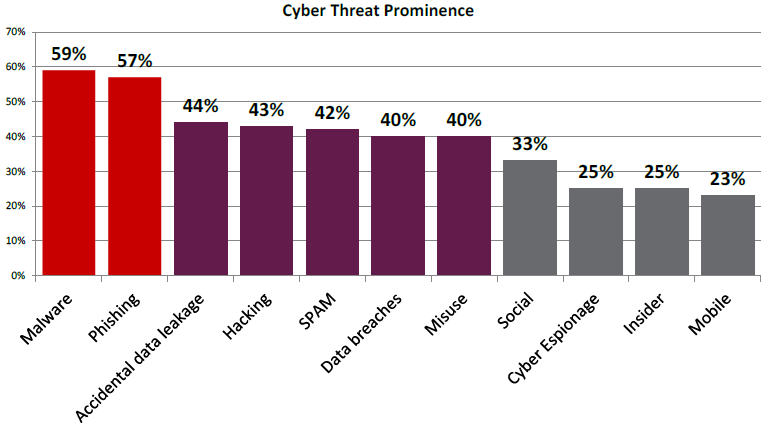
\includegraphics[width=0.55\paperwidth]{img1.png}
\caption{Proporción de cyber ataques}%\label{fig:horizonte}
\end{figure}

\end{columns}
\end{frame}

%------------------------------------------------
\section{Perfiles de amenazas (ii)}
%------------------------------------------------

\begin{frame}
\frametitle{Perfiles de amenazas (ii)}
\begin{columns}[c] % The "c" option specifies centered vertical alignment while the "t" option is used for top vertical alignment

\column{.35\textwidth} % Left column and width
\textbf{}
Las amenazas móviles son el vector emergente. Sólo el 44\% de todos los participantes en el estudio creen que están bien preparados, mientras que el 47\% dice que son algo preparados. Esta es la categoría de amenaza con el porcentaje más bajo de preparación combinada, y refleja la rapidez con que la informática móvil está superando los mecanismos de seguridad establecidos, técnicas y educación.


\column{.5\textwidth} % Right column and width
\begin{figure}[htb]
\centering
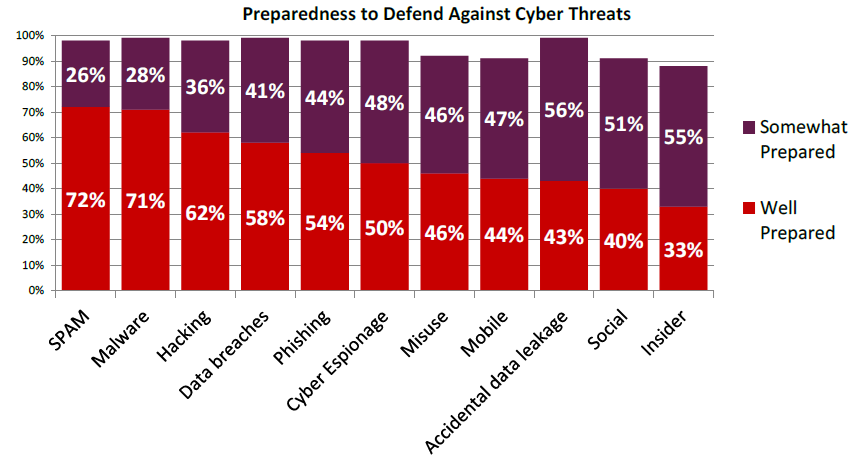
\includegraphics[width=0.50\paperwidth]{img2.png}
\caption{Preparación para defenderse ante cyber ataques}%\label{fig:horizonte}
\end{figure}

\end{columns}
\end{frame}

%------------------------------------------------

\section{Aplicaciones en Big Data (i)}
%------------------------------------------------

\begin{frame}
\frametitle{Ejemplo de aplicaciones en Big Data}
%\begin{columns}[c] % The "c" option specifies centered vertical alignment while the "t" option is used for top vertical alignment

%\column{.5\textwidth} % Right column and width
\begin{figure}[htb]
\centering
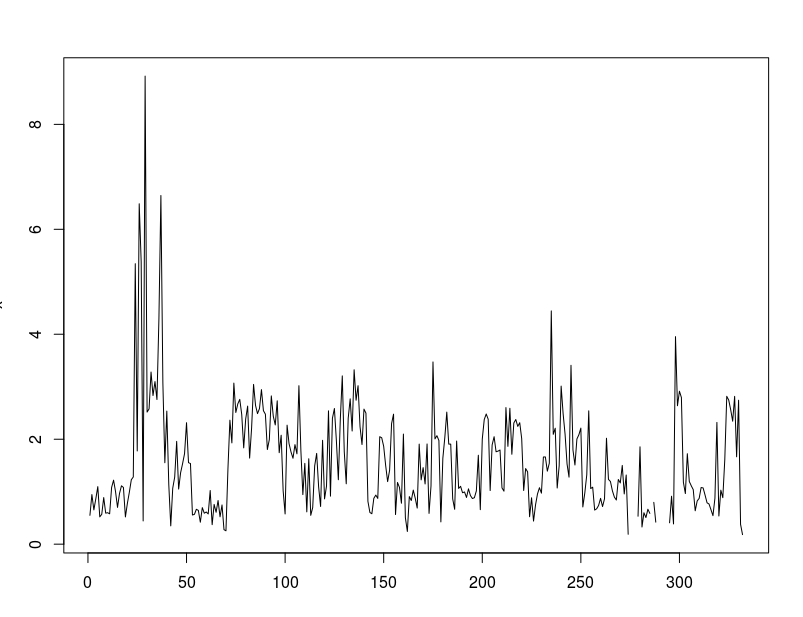
\includegraphics[width=0.50\paperwidth]{nitrate.png}
\caption{Variación de concentración de nitrato}%\label{fig:horizonte}
\end{figure}

%\end{columns}
\end{frame}

%------------------------------------------------

%------------------------------------------------

\section{Aplicaciones en Big Data (ii)}
%------------------------------------------------

\begin{frame}
\frametitle{Ejemplo de aplicaciones en Big Data}
%\begin{columns}[c] % The "c" option specifies centered vertical alignment while the "t" option is used for top vertical alignment

%\column{.5\textwidth} % Right column and width
\begin{figure}[htb]
\centering
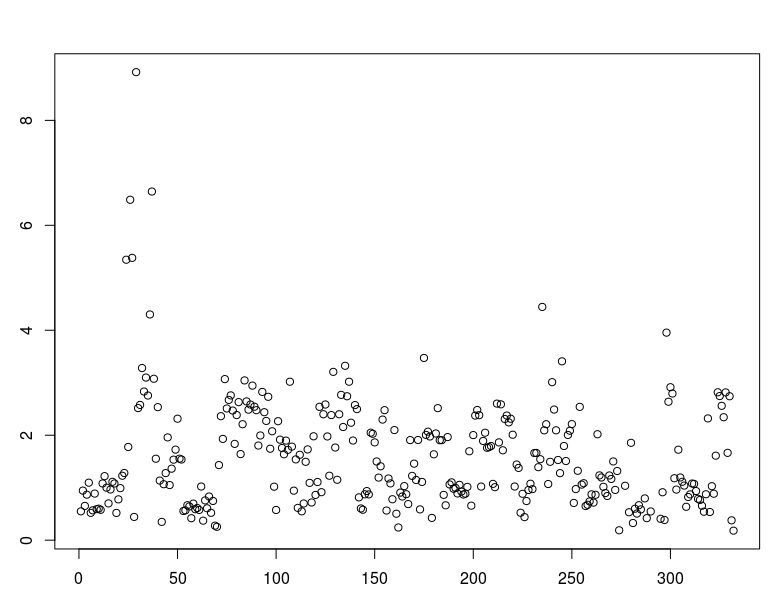
\includegraphics[width=0.50\paperwidth]{sulfate.png}
\caption{Variación de concentración de sulfato}%\label{fig:horizonte}
\end{figure}

%\end{columns}
\end{frame}


\begin{frame}
\frametitle{References}
\footnotesize{
\begin{thebibliography}{1}
\bibitem{unistan} Obrst, L., Chase, P., Markeloff, R., Developing an Ontology of the Cyber-security Domain, Semantic Technology for Intelligence, Defense and Security (STIDS) 2012, GMU, Fairfax, VA, 2012\\
\bibitem{brid} Big data: The next frontier for innovation, competition, and productivity. James Manyika, Michael Chui, Brad Brown, Jacques Bughin, Richard Dobbs, Charles Roxburgh, and Angela Hung Byers. McKinsey Global Institute. May 2011.\\
\bibitem{par} Using Data for Systemic Financial Risk Management. Mark Flood, H V Jagadish, Albert Kyle, Frank Olken, and Louiqa Raschid. Proc. Fifth Biennial Conf. Innovative Data Systems Research, Jan. 2011.\\
\bibitem{parallel} LM Cyber Security and Transformational Technologies Keeping Systems and Data Safe.\\
\bibitem{paralelo2} Big Data Analytics for Security Intelligence 2013 Cloud Security Alliance – All Rights Reserved.\\
\bibitem{parallel3} CV: Capital de riesgo; \url{https://es.wikipedia.org/wiki/Capital_riesgo}\\
\bibitem{parallel4} Cybersecurity is the killer app for big data analytics by Steve Morgan \url{http://www.csoonline.com/article/2942083/big-data-security/cybersecurity-is-the-killer-app-for-big-data-analytics.html}\\
\bibitem{parallel5} The 5 worst Big data privacy risks; \url{http://www.csoonline.com/article/2855641/big-data-security/the-5-worst-big-data-privacy-risks-and-how-to-guard-against-them.html} \\
\end{thebibliography}
}
\end{frame}

%------------------------------------------------

\begin{frame}
\Huge{\centerline{The End}}
\end{frame}

%----------------------------------------------------------------------------------------

\end{document}
